\section{Experiment 2: Acceptance of a Robot Programming Framework}

% \section{Can Users teach Action Models for Automated Planning using the Robot Programming Framework?}
\label{sec:Exp2}
%%%%%%%% 1.25 pages %%%%%%%

In this experiment, users were presented the robot programming framework (Sec. III), and had to teach action models by kinesthetic manipulation of a Baxter robot (Fig. \ref{fig:Baxter}). Users were instructed to demonstrate an atomic action and assign preconditions and effects. The goal was to assess the framework's usability and difficulties encountered, when teaching action models.

\subsection{Experimental Setup \& Participants}
We recruited 11 participants (7 male, 4 female), who were students and staff members at Universit\'{e} Grenoble Alpes. 6 participants reported programming experience with office productivity software (`beginner'), 2 had previously taken a programming course before (`advanced'), and 3 were pursuing studies in Computer Science (`expert').
%4 participants had previously heard of Automated Planning, but only 3 attended a related course.
The experiments were conducted using a Baxter robot (Fig. \ref{fig:Baxter}), mounted with a partial implementation of the framework (e.g. `learn a new action', `find an object', `execute an action sequence'). We used the Wizard-of-Oz technique to simulate the remaining functionalities (e.g. `generate action sequence').
Participants operated on a table with 2 positions (A and B), 2 cubes (blue and red), that represented parts on an assembly line. 
Each participant was allocated 1 hour, but the average duration was 29.5 minutes. The experiments were recorded, while the participant interacted with the robot. 

 
%The complete experimental protocol is shown in Fig. \ref{fig:Experimental protocol}. 
\subsection{Experimental Design \& Measurements}
The experiment was set in a simulated assembly line, where objects of the same shape, but different colour arrived consecutively at position A.
Users had to teach Baxter the action for moving an object from position A to position B, where objects should not be stacked. Throughout the experiment, users were faced with two different scenarios, where Baxter had to apply the learned action model. We evaluated the user's capability to refine action models, when faced with different situations, and wanted to assess the framework's overall usability.
The experiment consisted of the following phases:
\begin{itemize}
  %\item{Introduction: After a short introduction to the Baxter robot \cite{Baxter}, users were told that they needed to use a planning language (STRIPS) to explain Baxter the state of the world and the semantic meaning of the actions.}
  \item{\textbf{Training:} Users were shown how to manipulate Baxter's arm, and given time to familiarise themselves with the kinesthetic manipulation.}
  \item{\textbf{Experimental test:} Users were instructed to teach Baxter a move action of a cube. Then, they were presented the action model, with preconditions and effects, that Baxter learned from the demonstration (Fig. \ref{fig:scenarios-exp2}a). In the following, users were faced with two different scenarios, to refine the conditions of the action model. Starting with the initial action model for a red cube, users modified the conditions, so that it was applicable to all cubes of any colour (Fig. \ref{fig:scenarios-exp2}b), and when the target position was occupied (Fig. \ref{fig:scenarios-exp2}c). At each step, users observed how Baxter applied the learned action in the new scenario. When Baxter failed to execute the action, users had to refine the conditions of the action model.}
  \item{\textbf{Planning:} Users were presented a new scenario, where Baxter was instructed to achieve a new goal using the learned action model. The new goal was to switch the positions of two cubes on the table. Baxter demonstrated this by executing an action sequence generated by an automated planner.}
  \item{\textbf{Questionnaire:} Users were given a questionnaire containing 18 questions related to their experience (Fig. \ref{fig:eEvaluation}).}
   \item{ \textbf{Debriefing:} Users were questioned about their expectations on Baxter's behaviour, before applying the learned action model to a new scenario. Users were asked open-ended questions (``What will Baxter do when applying the learned action model?"), so that their responses were unbiased. When they encountered failure scenarios, they were asked to reason about Baxter's behaviour.} 
\end{itemize}

 \begin{figure}[t]
  \centering
  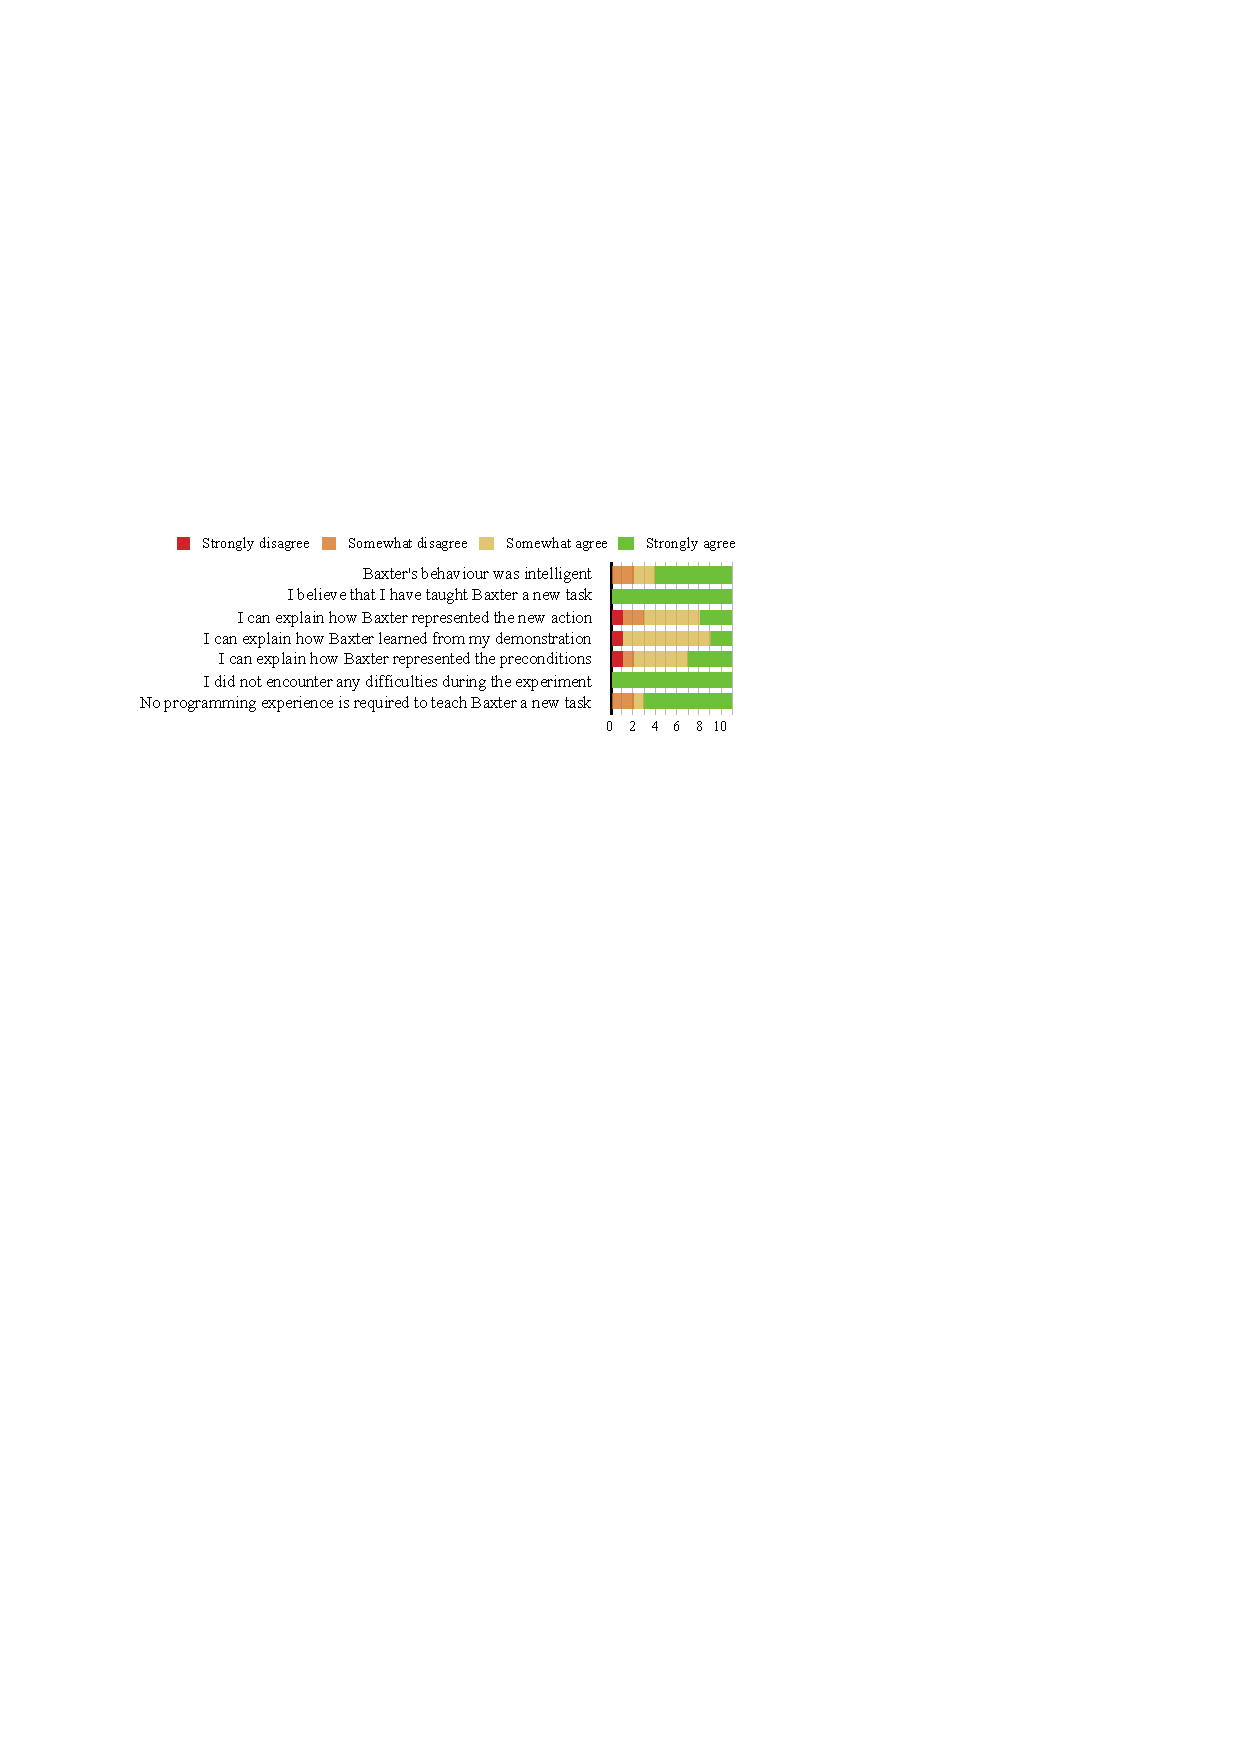
\includegraphics[width=8.7cm]{figures/eEvaluation1}
  \caption{Summary of questionnaire responses: Extract of 18 questions on the user's understanding, after the experiment to teach action models by demonstration (Sec. \ref{sec:Exp2}).}
  \label{fig:eEvaluation1}
\end{figure}



\todo{!! COMBINE ABOVE WITH OLDER VERSION BELOW !!}


\subsection{Problem statement}
Existing PbD implementations teach a robot a task execution, without their semantic meaning, and do not teach them goal-oriented behaviour. Automated planning solutions allow such behaviour, but require expert knowledge of PDDL and in first-order logic. With our proposed framework, we provide a way for non-expert users to create action models in PDDL by demonstration. We want to evaluate whether the logical concepts used in the two domains (PbD and Automated Planning) are usable for user groups without any programming knowledge.
The created action models need to have the correct preconditions and effects in order to be used in a goal-oriented approach using automated planners. For example, if the \texttt{drop} action does not have the precondition \texttt{empty ?l - location} -- meaning the location is unoccupied -- then the robot would try to place an object on an occupied space. Thus, it is important for the user to be able to understand and consider these conditions, when creating new action models. 

With this experiment, we aim to investigate whether the underlying logic of the chosen PDDL representation is appropriate for a user without programming experience to construct an action model.
We therefore simulate an environment, where our framework is fully functional, and the user is asked to teach the robot a new action by demonstration. As we aim to observe the users adoption of the notion of preconditions and effects, we decided to simulate the robot's learning process of a complete pick-and-place action, rather than individual pick, move and drop actions. The experiments allow us to evaluate the feasibility of implementing our framework and preempt any difficulties that may arise.

\subsection{Experimental set up}
We first considered using a real-life Tetris game to evaluate our framework and therefore manufactured the necessary elements (all Tetris pieces and 10x20 grid). However, since we target cobotic environments, this game does not seem appropriate to evaluate human-robot collaboration. We therefore chose the more realistic scenario of an assembly line in a manufacturing environment.

We first targeted user groups that were programming experts and had knowledge of automated planning techniques. We then focused on our main target group, which were users of different educational background and without programming experience.
Figure \ref{fig:Participants} shows the distribution of the participants recruited for the experimentation.
We recruited 11 subjects, 4 male and 7 female, and 5 with a background in science or technology. 3 subjects had an educational background in Computer Science, while 2 had previously taken a programming course and the remaining have only used productivity software. The subjects, who did not study Computer Science, had never used a robot that was able to pick up object by itself. Half of the subjects had previously heard of Automated Planning, out of which 3 have attended a related course.

%   \begin{figure}[h]
%     \centering
%     \includegraphics[scale=1]{figures/eParticipants}
%   \caption{Recruited participants}
%     \label{fig:Participants}
%   \end{figure}
The experiment was conducted using a Baxter Research Robot, equipped with the partial implementation of our framework. Since we did not manage to implement the whole framework, we simulated parts of its functionalities using the Wizard of Oz experimental approach \cite{kelley1985cal}. The object detection method, trajectory learning process and final task execution were demonstrated using our implementation. We simulated the reproduction of the demonstrated action, as well as the robot's learning of the observed predicates. Moreover, to incorporate human-relatable behaviours, we simulated social feedback cues into the Baxter's interaction with the subject (e.g. Baxter shakes its head to signal refusal of a pick-and-place action, and nods to signal approval of a learned action).

The surface of the table consists of a grid, with 2 separate positions marked with A and D (arrival and departure respectively). The objects on the table are two square blocks (red and blue), that represent parts on an assembly line (see Figure \ref{fig:Experimental set up}). The subjects operate Baxter's right limb, equipped with a camera and a suction gripper, that can manipulate one block at a time. During Baxter's search action, the limb camera is projected to Baxter's screen, allowing the subject to observe the action process. Throughout the experiment, the subject is presented with action models that represent Baxter's learned \texttt{pick-and-place} action (see Appendix A3). The subject is guided and questioned by the experimenter. At the end of the experiment, the subject is given a questionnaire to complete (see Appendix A3). All experiments were conducted in French, thus, the supporting material (questionnaire, schema of action models, protocol) were created in French as well. The experiment is recorded while the subject interacts with the robot, until they are given the questionnaire at the end. Each session was allocated 1 hour, but in the end each session took an average of 29 minutes and 32 seconds.

\begin{figure}[h]
\centering
\begin{minipage}{0.5\textwidth}
  \centering
    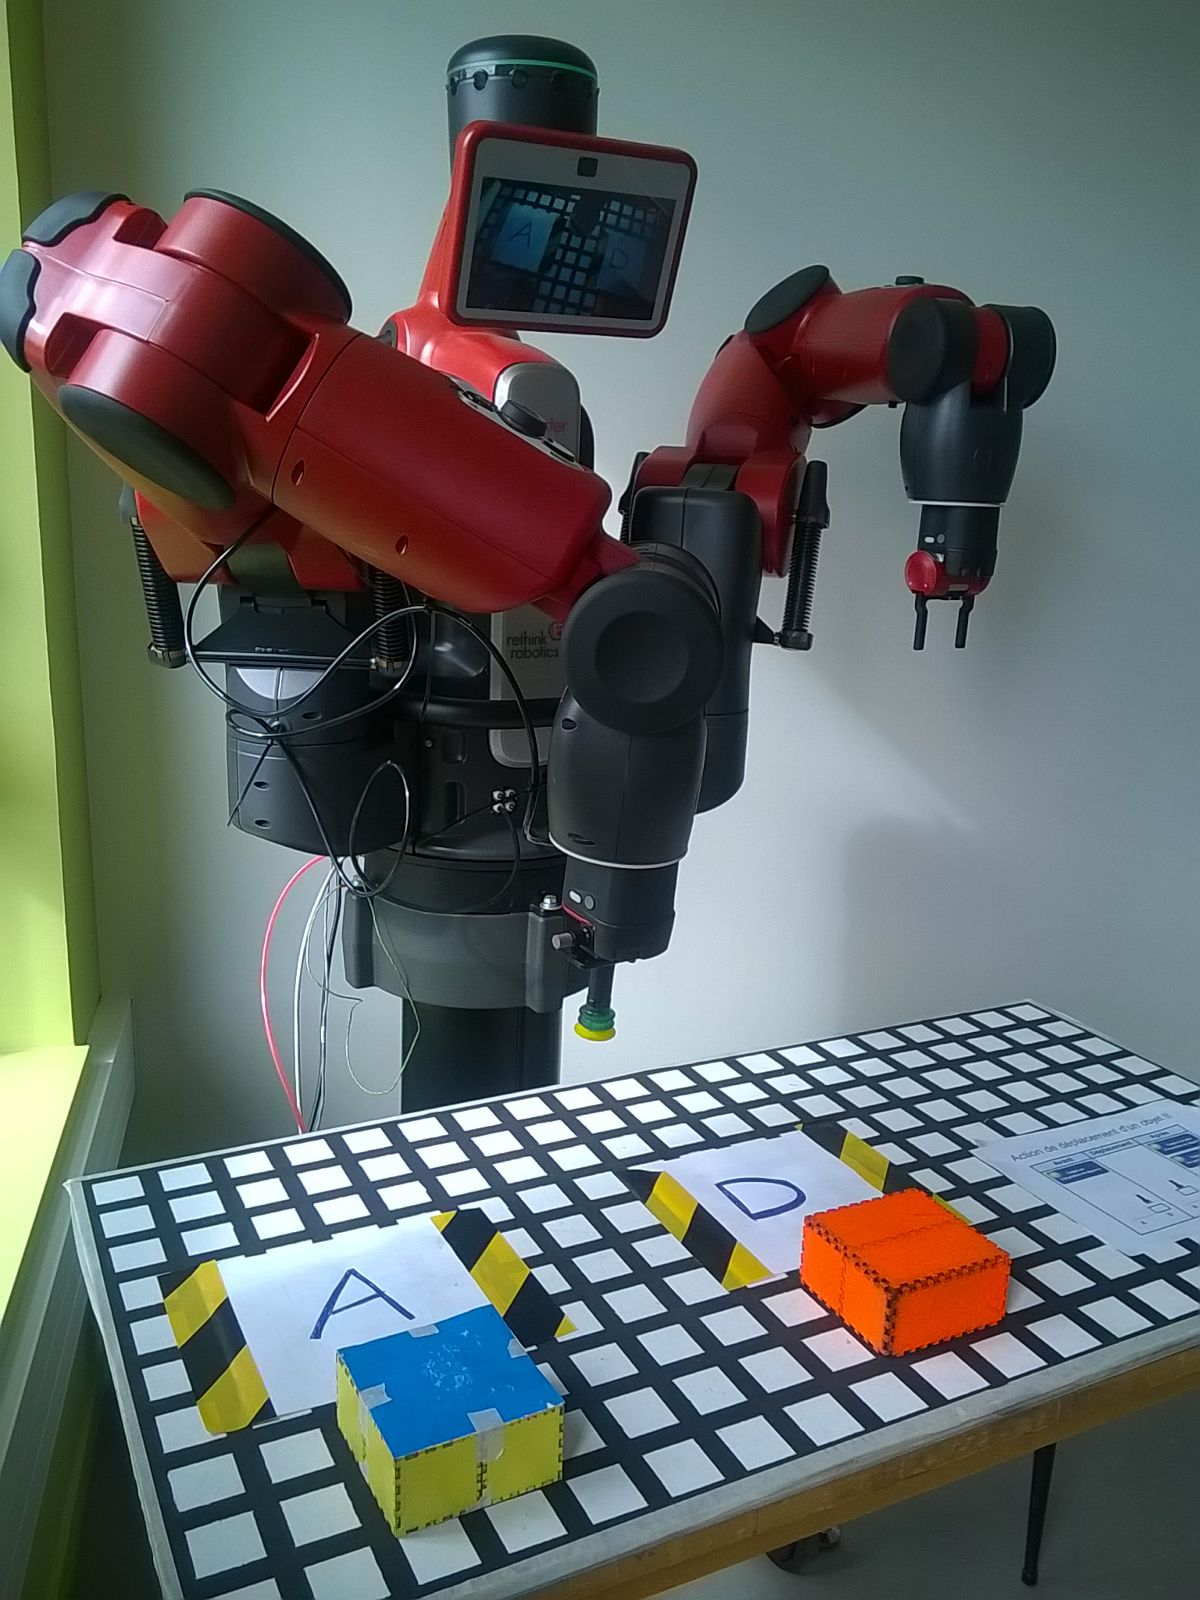
\includegraphics[scale=0.2]{figures/experiment}
    \caption{Experimental set up}
    \label{fig:Experimental set up}
\end{minipage}%
\begin{minipage}{.5\textwidth}
  \centering
    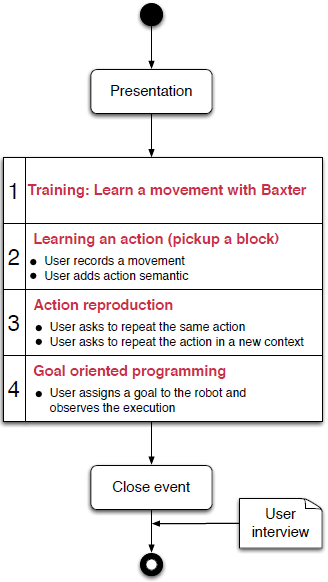
\includegraphics[scale=0.56]{figures/protocole}
    \caption{Experimental design}
    \label{fig:Experimental design}
\end{minipage}
\end{figure}

\subsection{Principle Hypotheses}
We have set the following principle hypotheses for our experiments:
\begin{enumerate}
\item A user without any programming knowledge is able to teach Baxter a pick-and-place action to fulfill a task.
\item The user understands the concepts of actions, preconditions, and effects.
\item The user perceives Baxter as having learned a new task.
\end{enumerate}

\subsection{Experimental design \& Protocol}
We aimed to find a domain that was simple enough to introduce new information and to test the subject's capability of understanding it in a relatively short amount of time. The experiment takes place in a simulated assembly line, where objects of the same shape but different colour arrive consecutively at a zone D (for departure). Objects are assumed to be dangerous or too heavy, similar to manufacturing environments, and should not be stacked. Baxter knows how to search for an object on the table using the camera on its arm. Furthermore, it can learn new actions using our implemented framework. The subject is asked to teach Baxter the action for picking up an object from zone D and placing it at zone A (for arrival) by manipulating Baxter's arm and using the suction gripper. We subsequently introduce the subject to the action model representation of preconditions and effects and test their understanding thereof. We start with a simple representation, which is not applicable for all scenarios, and guide the subject towards a generalised representation. The subject is regularly questioned about their observations and assumptions on Baxter's behaviour (\textit{Briefing}).
Figure \ref{fig:Experimental design} shows the experimental design.


\subsection{Training}
The subject is first introduced to the experimenter's project and presented the Baxter robot in real-life applications by showing a video of Baxter operating in a manufacturing environment \cite{BaxterYoutube}. The subject is subsequently introduced to the simulation scenario of being the human operator on an assembly line, required to teach Baxter how to pick-and-place an object. The experimenter shows the subject how to operate Baxter's arm and activate the suction gripper to pick up and object. The subject replicates the demonstrated action multiple times to familiarise themselves with the robot and the arm manipulation. Despite initial difficulties, all of the participants managed to operate Baxter's arm without any problems and stated that the manipulation was simple. On average, the training session took 2 minutes and 43 seconds.

\subsection{Learning an action}
When the subject has familiarised themselves with the arm manipulation, the experimental phase starts. The subject is made aware that it will teach Baxter a pick-and-place action by demonstrating the movement. The experimenter commands Baxter to record the demonstrated movement, with Baxter signaling the beginning and ending of the learning process by nodding its head. The experimenter commands Baxter to reproduce the learned action and the subject is asked to validate that the action has been learned correctly. The majority of subjects confirmed that the action was learned well. Then, the subject is presented the observed conditions (preconditions and effects of the pick-and-place action) that Baxter has learned from the action demonstration (see Schema I in Appendix A3).
The subject verifies that the conditions are correct for the learned action. All subjects stated that the conditions were correct for the taught pick-and-place action and found this representation easy to understand. When questioned about any suggested improvements, none of the participants proposed a generalised model (without the colour) or an additional condition.

\begin{table}[h]
\begin{center}
\begin{tabular}{l|l}
Preconditions & Effects\\ \hline
 & \\
The red object is at initial position D. & The red object is at goal position A.\\
 & The red object is not at initial position D.
\end{tabular}
\end{center}
\label{tab:schema1}
\caption{Schema of action model I}
\end{table}

\subsection{Action reproduction}
The subject was then introduced to a new context, where Baxter has to reproduce the pick-and-place action with a blue object, instead of a red one. The subject was questioned about the robot's expected behaviour. 6 out of 11 subjects responded correctly that Baxter will not be able to execute the action with the learned action model.
Baxter is then commanded to reproduce the pick-and-place action, but refuses by shaking its head. The subject is questioned about the robot's reasoning and possible improvements to create a generic action model. All subjects pointed out that the colour was the problem. 8 out of 11 subjects deduced that the colour should not be taken into consideration, whereas the remaining 3 suggested to teach Baxter the same action with the blue object. The subjects were presented the updated action model (see Schema II in Appendix A3) and questioned about any improvements to add. At this stage, all subjects were content and did not propose any modifications.
\begin{table}[h]
\begin{center}
\begin{tabular}{l|l}
Preconditions & Effects\\ \hline
 & \\
The object is at initial position D. & The object is at goal position A.\\
 & The object is not at initial position D.
\end{tabular}
\end{center}
\label{tab:schema2}
\caption{Schema of action model II}
\end{table}

The second scenario is a continuation of the simulated assembly line, where the blue object occupies the arrival zone A and a red object is placed on the departure zone D. The subjects were again questioned about the robot's expected behaviour, considering its learned action model. 6 out of 11 subjects predicted correctly that Baxter will stack the two objects with the learned action model. Baxter executes the learned action by stacking the two objects, therefore violating the constraint of our simulated environment. All subjects noted the reason for the robot's behaviour as being a missing condition in the robot's action model and stated that the robot should not do anything while the arrival zone was occupied. Only 5 out of 11 subjects stated explicitly that the missing condition was for the arrival zone A to be empty. The subjects were presented the updated action model (see Schema III in Appendix A3).
\begin{table}[h]
\begin{center}
\begin{tabular}{l|l}
Preconditions & Effects\\ \hline
 & \\
The object is at initial position D. & The object is at goal position A.\\
The goal position A is empty. & The object is not at initial position D.
\end{tabular}
\end{center}
\label{tab:schema3}
\caption{Schema of action model III}
\end{table}

\subsection{Goal-oriented programming}
The final phase in our experimentation introduces a different scenario on the assembly line, where Baxter has to permutate two objects that arrived in the wrong order. The subject was reminded that Baxter knows how to recognise objects on the table and was taught the action to pick and place an object in the previous phase. As previously, the subjects were questioned about the robot's expected behaviour in the given scenario, in particular, if the robot will succeed at accomplishing the task. The subjects were not informed that Baxter was connected to an automated planner. 3 out of 11 subjects responded correctly that Baxter will be able to perform the permutation by placing one object on the side in order to empty an occupied zone. The remaining subjects were not convinced that Baxter would be capable of performing the permutation and were therefore asked to demonstrate the permutation themselves with only one arm. All of the participants placed an object on the side to empty one of the two goal positions. After commanding Baxter to perform the permutation, it successfully permutated the two objects by following the same reasoning. All subjects stated that they found Baxter's behaviour intelligent.

\subsection{User interview}
The final stage of the experiment consisted of a questionnaire. Figure \ref{fig:Participants} and Figure \ref{fig:eEvaluation} show an overview of the responses.
3 of the subjects that are studying Computer Science had already heard of Automated Planning in lectures and encountered no difficulties in understanding the concepts of preconditions and effects.
Subjects, that ranked themselves as having limited experience in Computer Science and had no knowledge about Automated Planning, found it easy to understand the concept of preconditions and effects.
All subjects encountered no difficulties when manipulating Baxter's arm and agreed that it was well adapted to workers in manufacturing environments.
At the end of the experiment, all subjects agreed that Baxter's behaviour in the final phase was intelligent. The majority of subjects were of the opinion that they had taught Baxter a new task (to move an object) and that they could explain how Baxter learned the new task by demonstration. Similarly, the majority of subjects stated that they could explain how Baxter represented the new task and the preconditions.
The majority of the subjects agreed that no programming knowledge was required to teach Baxter a new task. None of the subjects encountered any difficulties during the experiment.

  \begin{figure}[ht]
   \centering
    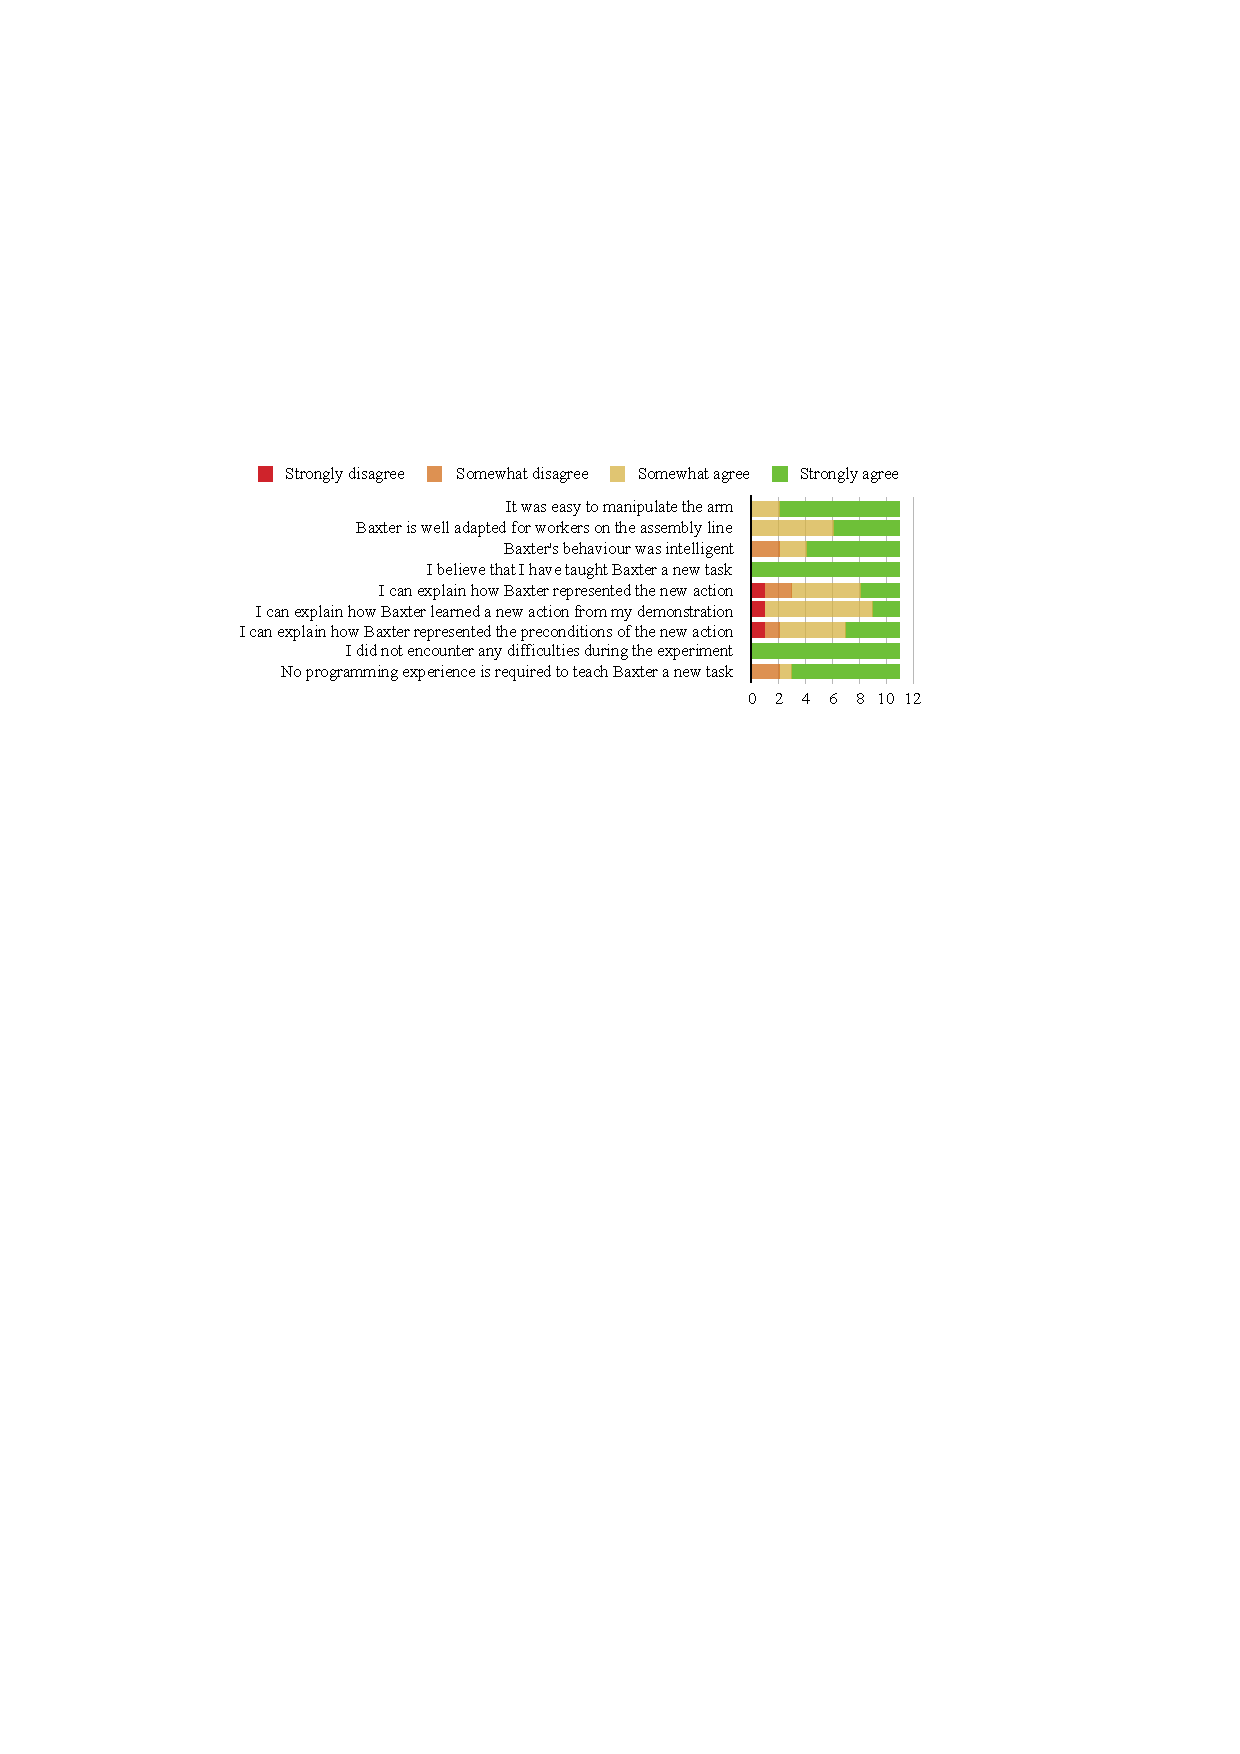
\includegraphics[scale=1]{figures/eEvaluation}
    \caption{Overview of responses to the questionnaire}
    \label{fig:eEvaluation}
\end{figure}

\subsection{Discussion and Conclusion}
%%%%%%%%%%%%%%%%%%%%%%%%%%%%%%%%%%%%%%%%%%%%%%%%%%%%%%%%%%%%%%%%%%%%%%%%%%%%%%%%
\subsubsection{Results}
%%%%%%%%%%%%%%%%%%%%%%%%%%%%%%%%%%%%%%%%%%%%%%%%%%%%%%%%%%%%%%%%%%%%%%%%%%%%%%%%
All (11) users were satisfied with the PbD process and Baxter's abilities to learn and reproduce the demonstrated move action. All users understood the learned action model and managed to adopt the notion of preconditions and effects easily. As expected, no users pointed out the missing conditions (Fig. \ref{fig:scenarios-exp2}c), when asked for improvements of the initial action model (Fig. \ref{fig:scenarios-exp2}a).
Even users who were `experts' and who had heard of automated planning before, did not manage to create a complete action model from the start. However, all users detected the missing condition easily, when faced with the relevant failure scenarios.

In the final phase, users with no experience in automated planning (8) did not expect Baxter to solve the permutation problem, and agreed unanimously that it acted in an intelligent manner, when it did. At the end of the experiment, all users believed that they had taught Baxter a new task and the majority understood the representation of the action models well. No users encountered any difficulties during the experiment. 8 participants believed that no programming experience was required to teach Baxter a task (Fig. \ref{fig:eEvaluation}).

\todo{!! COMBINE ABOVE WITH OLDER VERSION BELOW !!}

The aim of this experiment was to evaluate the performance of our framework with users with varying educational background. In particular, we wanted to find out if users understood the concept of robot programming by demonstration and the robot's learning procedure, by letting them teach Baxter a new action. Secondly, we aimed at evaluating the user's understanding of the representations in terms of preconditions and effects, commonly used in automated planning techniques. Finally, we wanted to identify any difficulties that the user's were facing throughout the experiment.

Overall, participants were satisfied with the learning by demonstration process and understood Baxter's learning abilities. All subjects understood the concept and notion of precondition and effects, associated with the learning process. As expected, no subjects managed to point out the missing conditions right at the start, but all subjects detected them, when faced with the relevant failure scenarios. However, the majority of subjects had difficulties in formulating the missing precondition (\textit{``zone A is empty"}) and suggested other equivalent conditions (\textit{``Do not place the object on zone A, if it is occupied"}). We conclude that the user interface should propose the user a pre-defined set of conditions that can be added to the action model.

We noted that throughout the experiment, some users made wide assumptions about the robot's capabilities. In our simulated environment, we set the constraint of not being allowed to stack two objects. In the scenario, where both arrival and departure zones were occupied, almost half of the subjects assumed that Baxter would not stack the two objects and consider the constraint, even though it was not mentioned in the Baxter's action model.
This is a common problem in PbD solutions as there is a difference in the perception of the robot's intelligence perceived by its teacher \cite{suay2012practical}. This can be easily addressed by reproducing the learned task in a new context and verifying the robot's intelligence as we did throughout the experiment.

On the other hand, subjects, which had no experience in automated planning, did not expect Baxter to execute the permutation task successfully, but agreed unanimously that it acted in an intelligent manner. At the end of the experiment, all subjects stated that they had taught Baxter a new task and that they understood the representation of the action models well. With this experiment we showed that the level of representing an action in terms of preconditions and effects is adequate for users in cobotic environments to teach a robot a new task by demonstration. 


%
%\subsection{Evaluation criteria}
%
%To Do: Describe the evaluation criteria used to analyse results of experiments, specifically the notion of success and failures.
%First problem of learning an atomic action from human demonstration:
%define an experiment as successful iff 
%robot learns correct task representation
%reproduces the task correctly
%performs tasks in changed environments (different objects/locations)
%
%Second challenge enables the robot to reach a goal by executing an action sequence produced by the automated planner.


%The user needs to communicate preconditions, effects and parameters relevant to the performed action for the operator to enter into the system. Baxter demonstrates the learned action to the user, who is asked about his understanding of the robot's learning of the taught movement. 
